\documentclass{article}\usepackage[]{graphicx}\usepackage[]{color}
%% maxwidth is the original width if it is less than linewidth
%% otherwise use linewidth (to make sure the graphics do not exceed the margin)
\makeatletter
\def\maxwidth{ %
  \ifdim\Gin@nat@width>\linewidth
    \linewidth
  \else
    \Gin@nat@width
  \fi
}
\makeatother

\definecolor{fgcolor}{rgb}{0.345, 0.345, 0.345}
\newcommand{\hlnum}[1]{\textcolor[rgb]{0.686,0.059,0.569}{#1}}%
\newcommand{\hlstr}[1]{\textcolor[rgb]{0.192,0.494,0.8}{#1}}%
\newcommand{\hlcom}[1]{\textcolor[rgb]{0.678,0.584,0.686}{\textit{#1}}}%
\newcommand{\hlopt}[1]{\textcolor[rgb]{0,0,0}{#1}}%
\newcommand{\hlstd}[1]{\textcolor[rgb]{0.345,0.345,0.345}{#1}}%
\newcommand{\hlkwa}[1]{\textcolor[rgb]{0.161,0.373,0.58}{\textbf{#1}}}%
\newcommand{\hlkwb}[1]{\textcolor[rgb]{0.69,0.353,0.396}{#1}}%
\newcommand{\hlkwc}[1]{\textcolor[rgb]{0.333,0.667,0.333}{#1}}%
\newcommand{\hlkwd}[1]{\textcolor[rgb]{0.737,0.353,0.396}{\textbf{#1}}}%
\let\hlipl\hlkwb

\usepackage{framed}
\makeatletter
\newenvironment{kframe}{%
 \def\at@end@of@kframe{}%
 \ifinner\ifhmode%
  \def\at@end@of@kframe{\end{minipage}}%
  \begin{minipage}{\columnwidth}%
 \fi\fi%
 \def\FrameCommand##1{\hskip\@totalleftmargin \hskip-\fboxsep
 \colorbox{shadecolor}{##1}\hskip-\fboxsep
     % There is no \\@totalrightmargin, so:
     \hskip-\linewidth \hskip-\@totalleftmargin \hskip\columnwidth}%
 \MakeFramed {\advance\hsize-\width
   \@totalleftmargin\z@ \linewidth\hsize
   \@setminipage}}%
 {\par\unskip\endMakeFramed%
 \at@end@of@kframe}
\makeatother

\definecolor{shadecolor}{rgb}{.97, .97, .97}
\definecolor{messagecolor}{rgb}{0, 0, 0}
\definecolor{warningcolor}{rgb}{1, 0, 1}
\definecolor{errorcolor}{rgb}{1, 0, 0}
\newenvironment{knitrout}{}{} % an empty environment to be redefined in TeX

\usepackage{alltt}
\usepackage{fullpage}
\usepackage{hyperref}
\IfFileExists{upquote.sty}{\usepackage{upquote}}{}
\begin{document}
\setlength{\parindent}{0cm}


\section{Install R}

R does have a static url address. There is no direct link to the download file. Please follow the steps below:\bigskip

1) Visit the main website  of the R software here: \url{http://r-project.org}.\bigskip

2) Click on CRAN link. CRAN is the network of servers which host R and R libraries.

\begin{figure}[!h]
 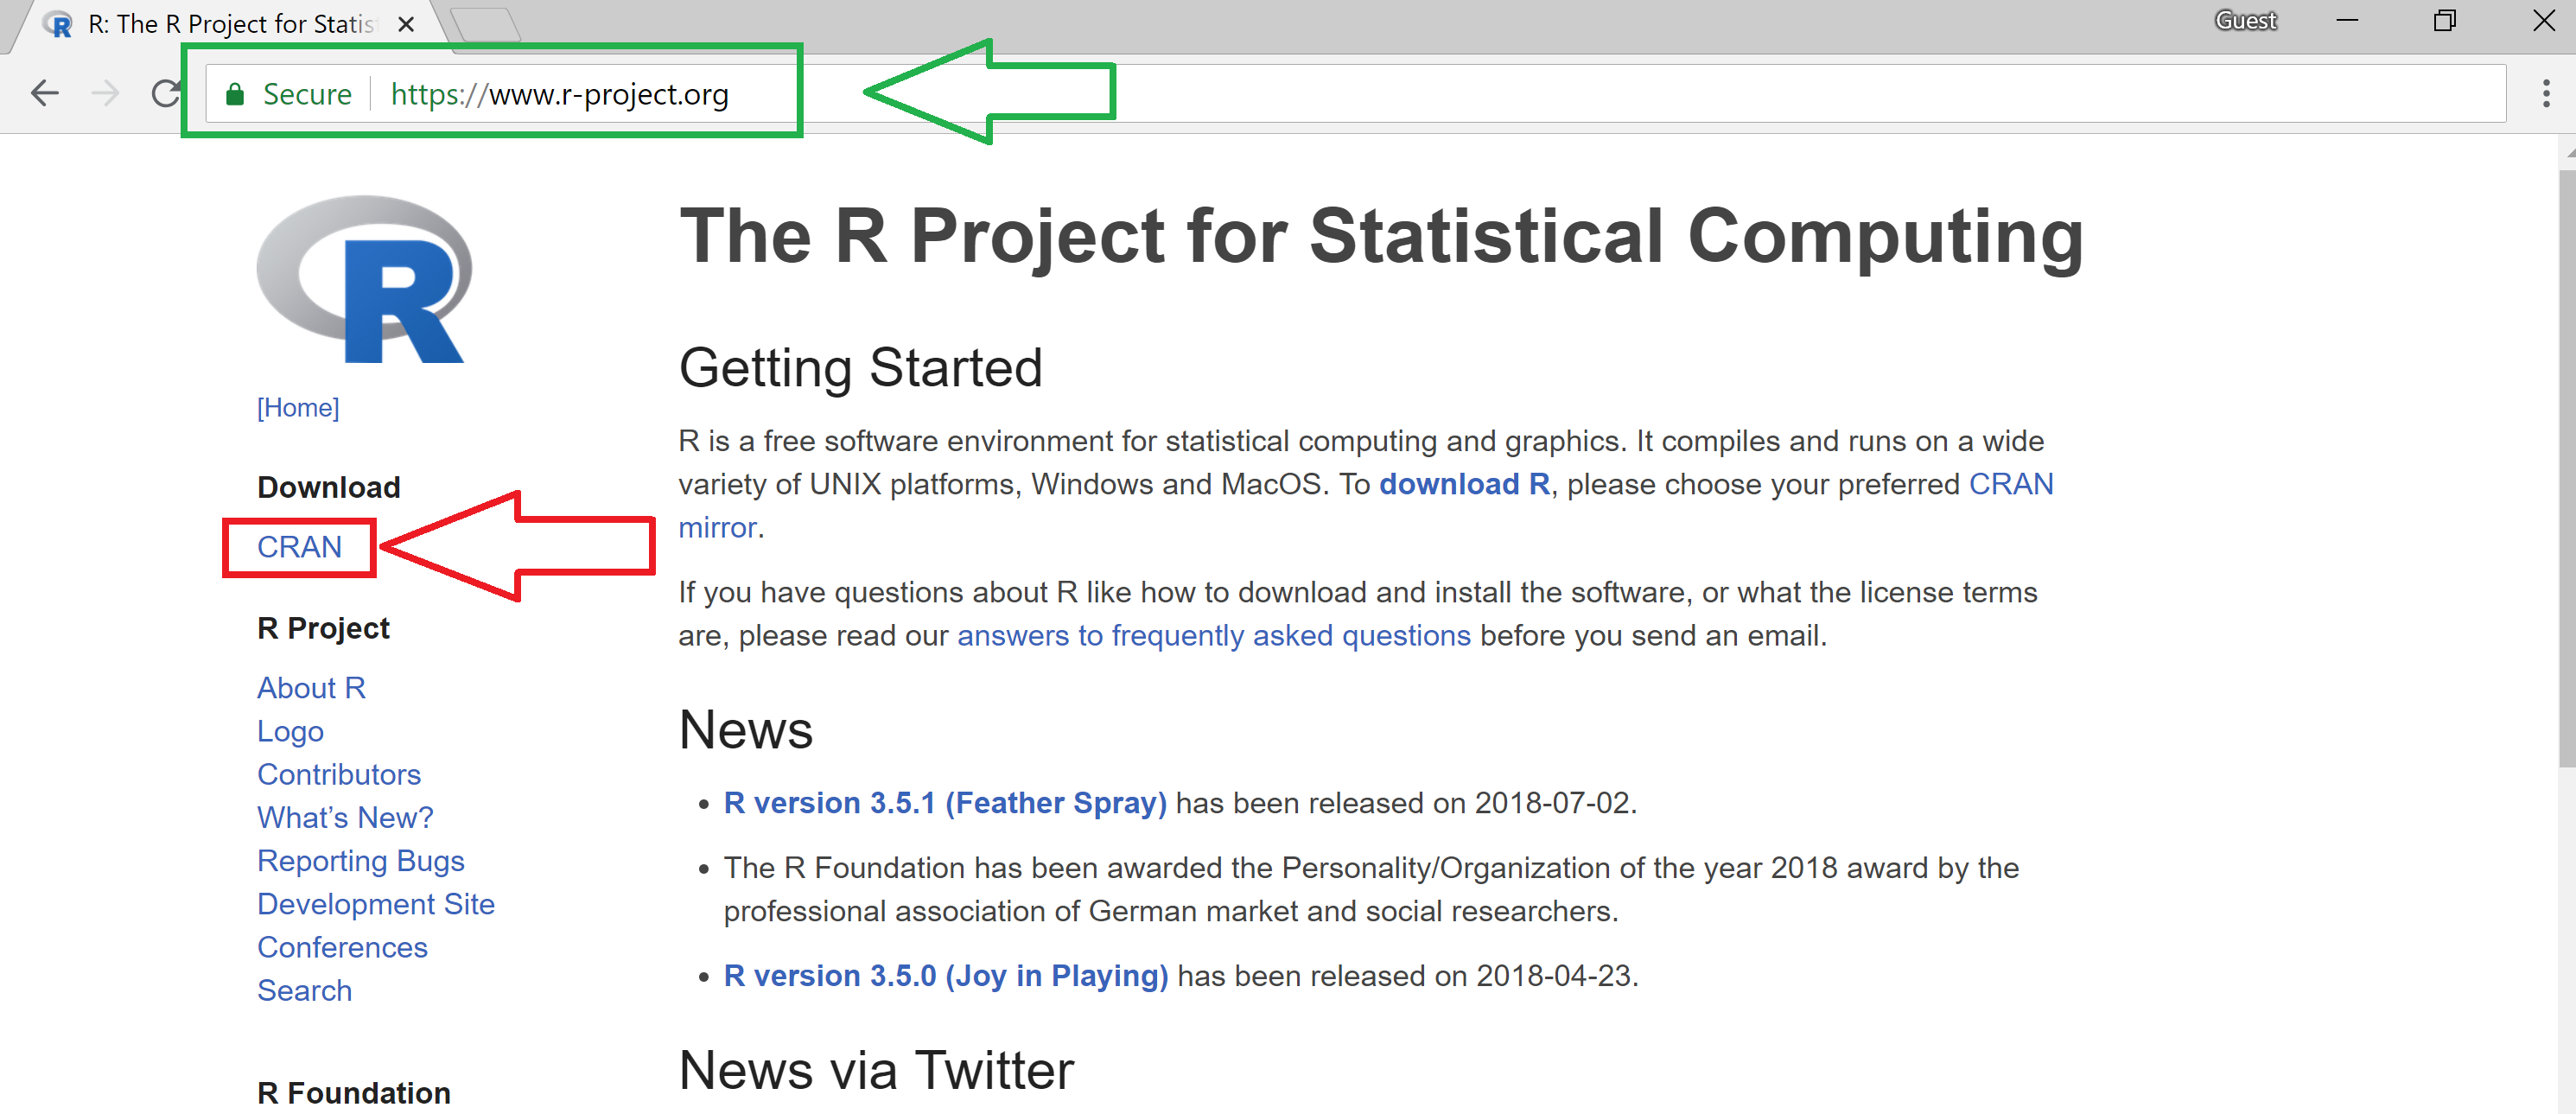
\includegraphics[width=\textwidth,height=\textheight,keepaspectratio]{./Images/image_01.png}
\end{figure}

3) CRAN network is scattered around the world. All have identical content (there is no Czech or Chinese verion of R). Selection of server influences download speed. The first option \texttt{0-Cloud} finds the most convenient option for you automatically.

\begin{figure}[!h]
 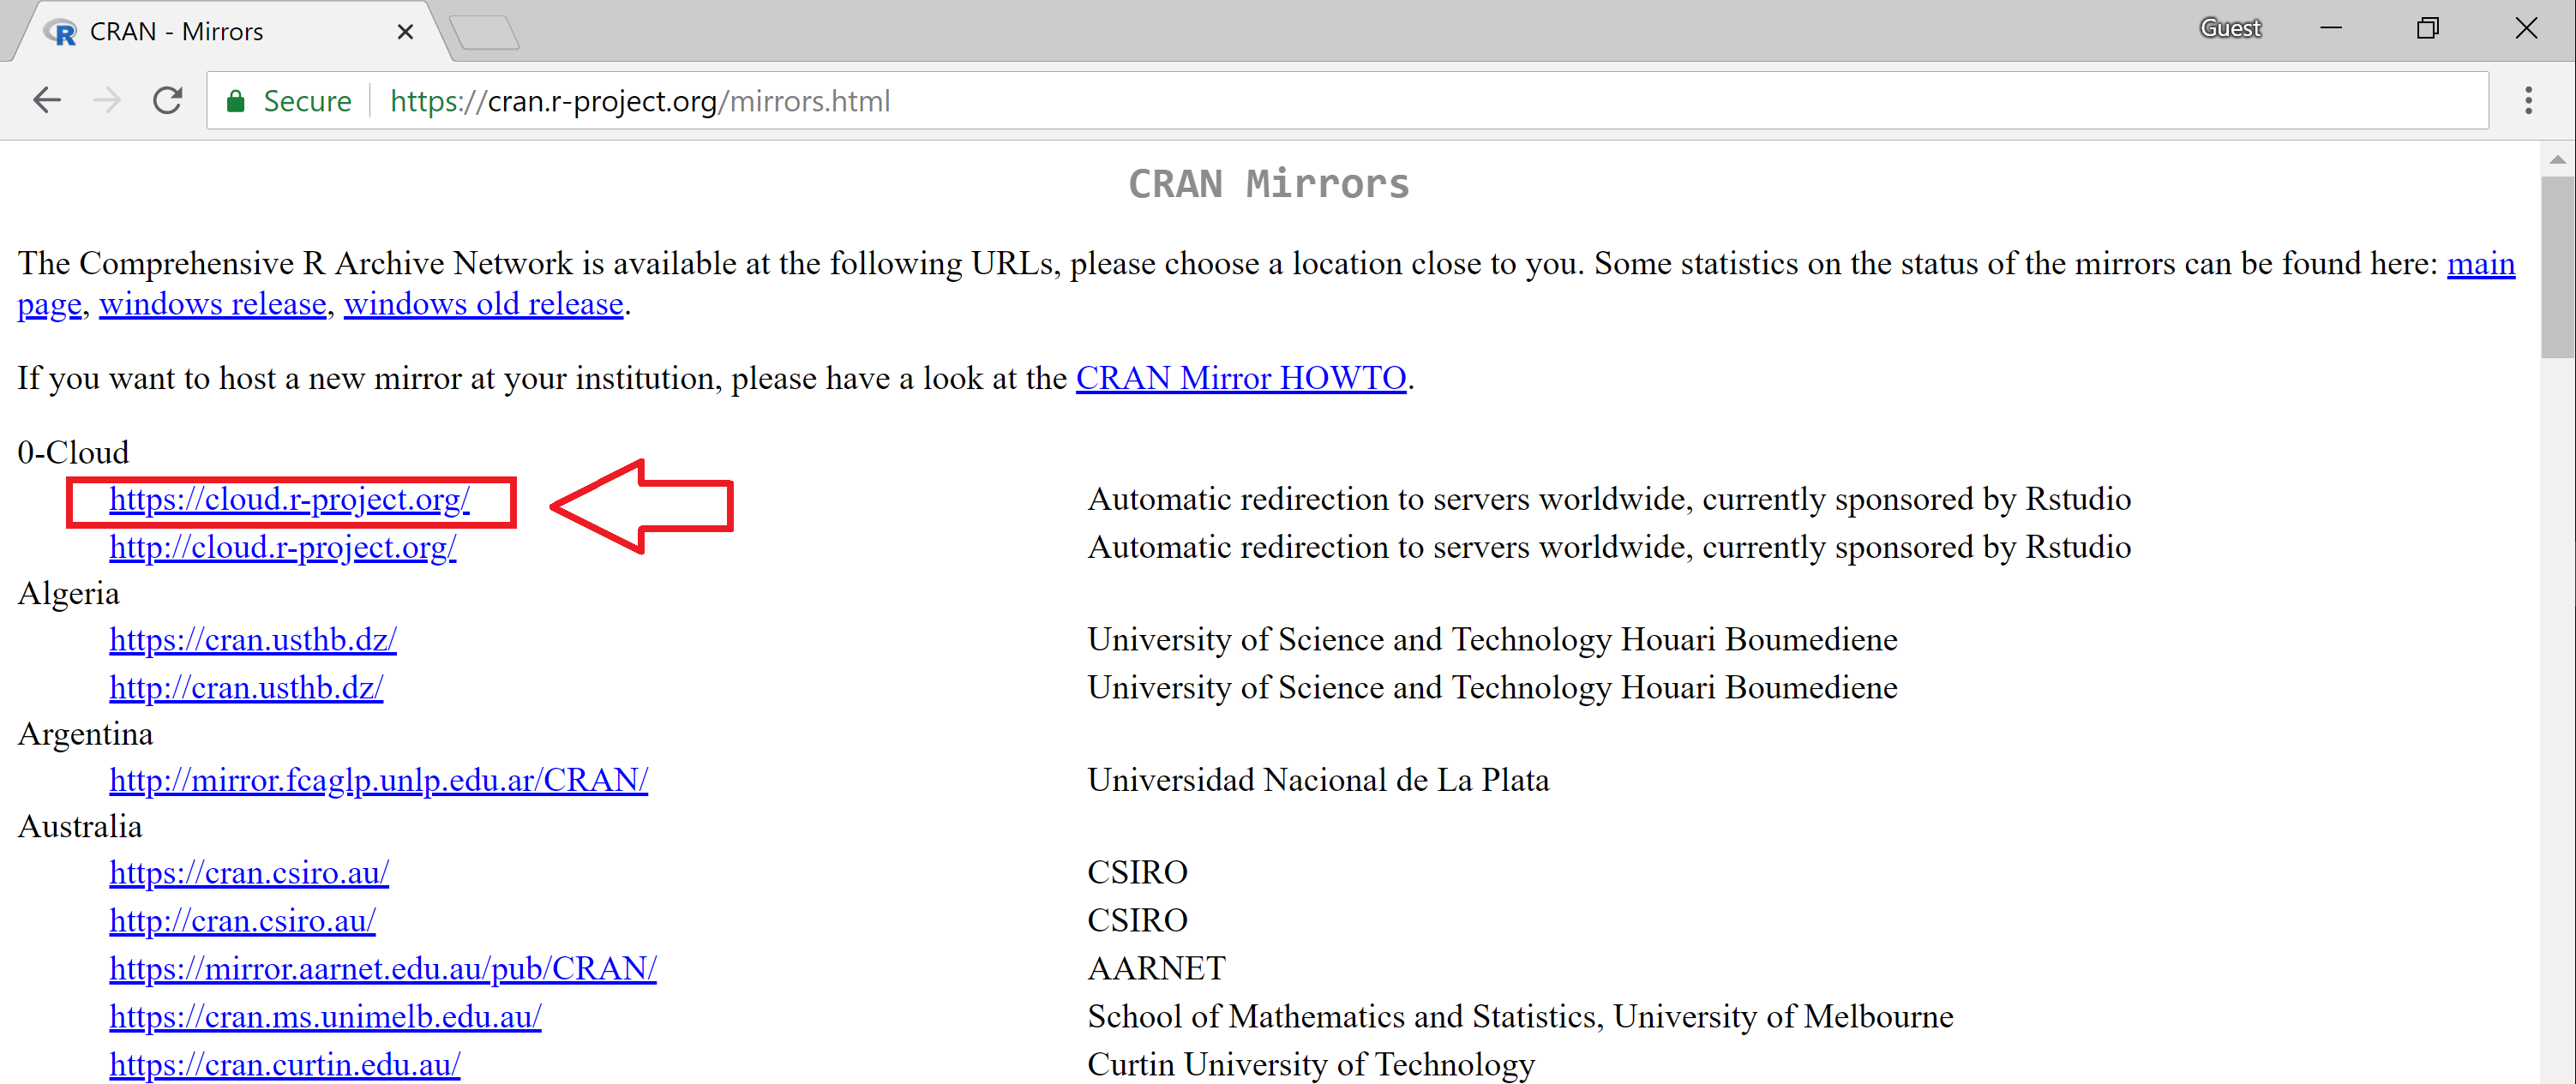
\includegraphics[width=\textwidth,height=\textheight,keepaspectratio]{./Images/image_02.png}
\end{figure}
\clearpage
4) Choose an appropriate R according to the platform you use. 

\begin{figure}[!h]
 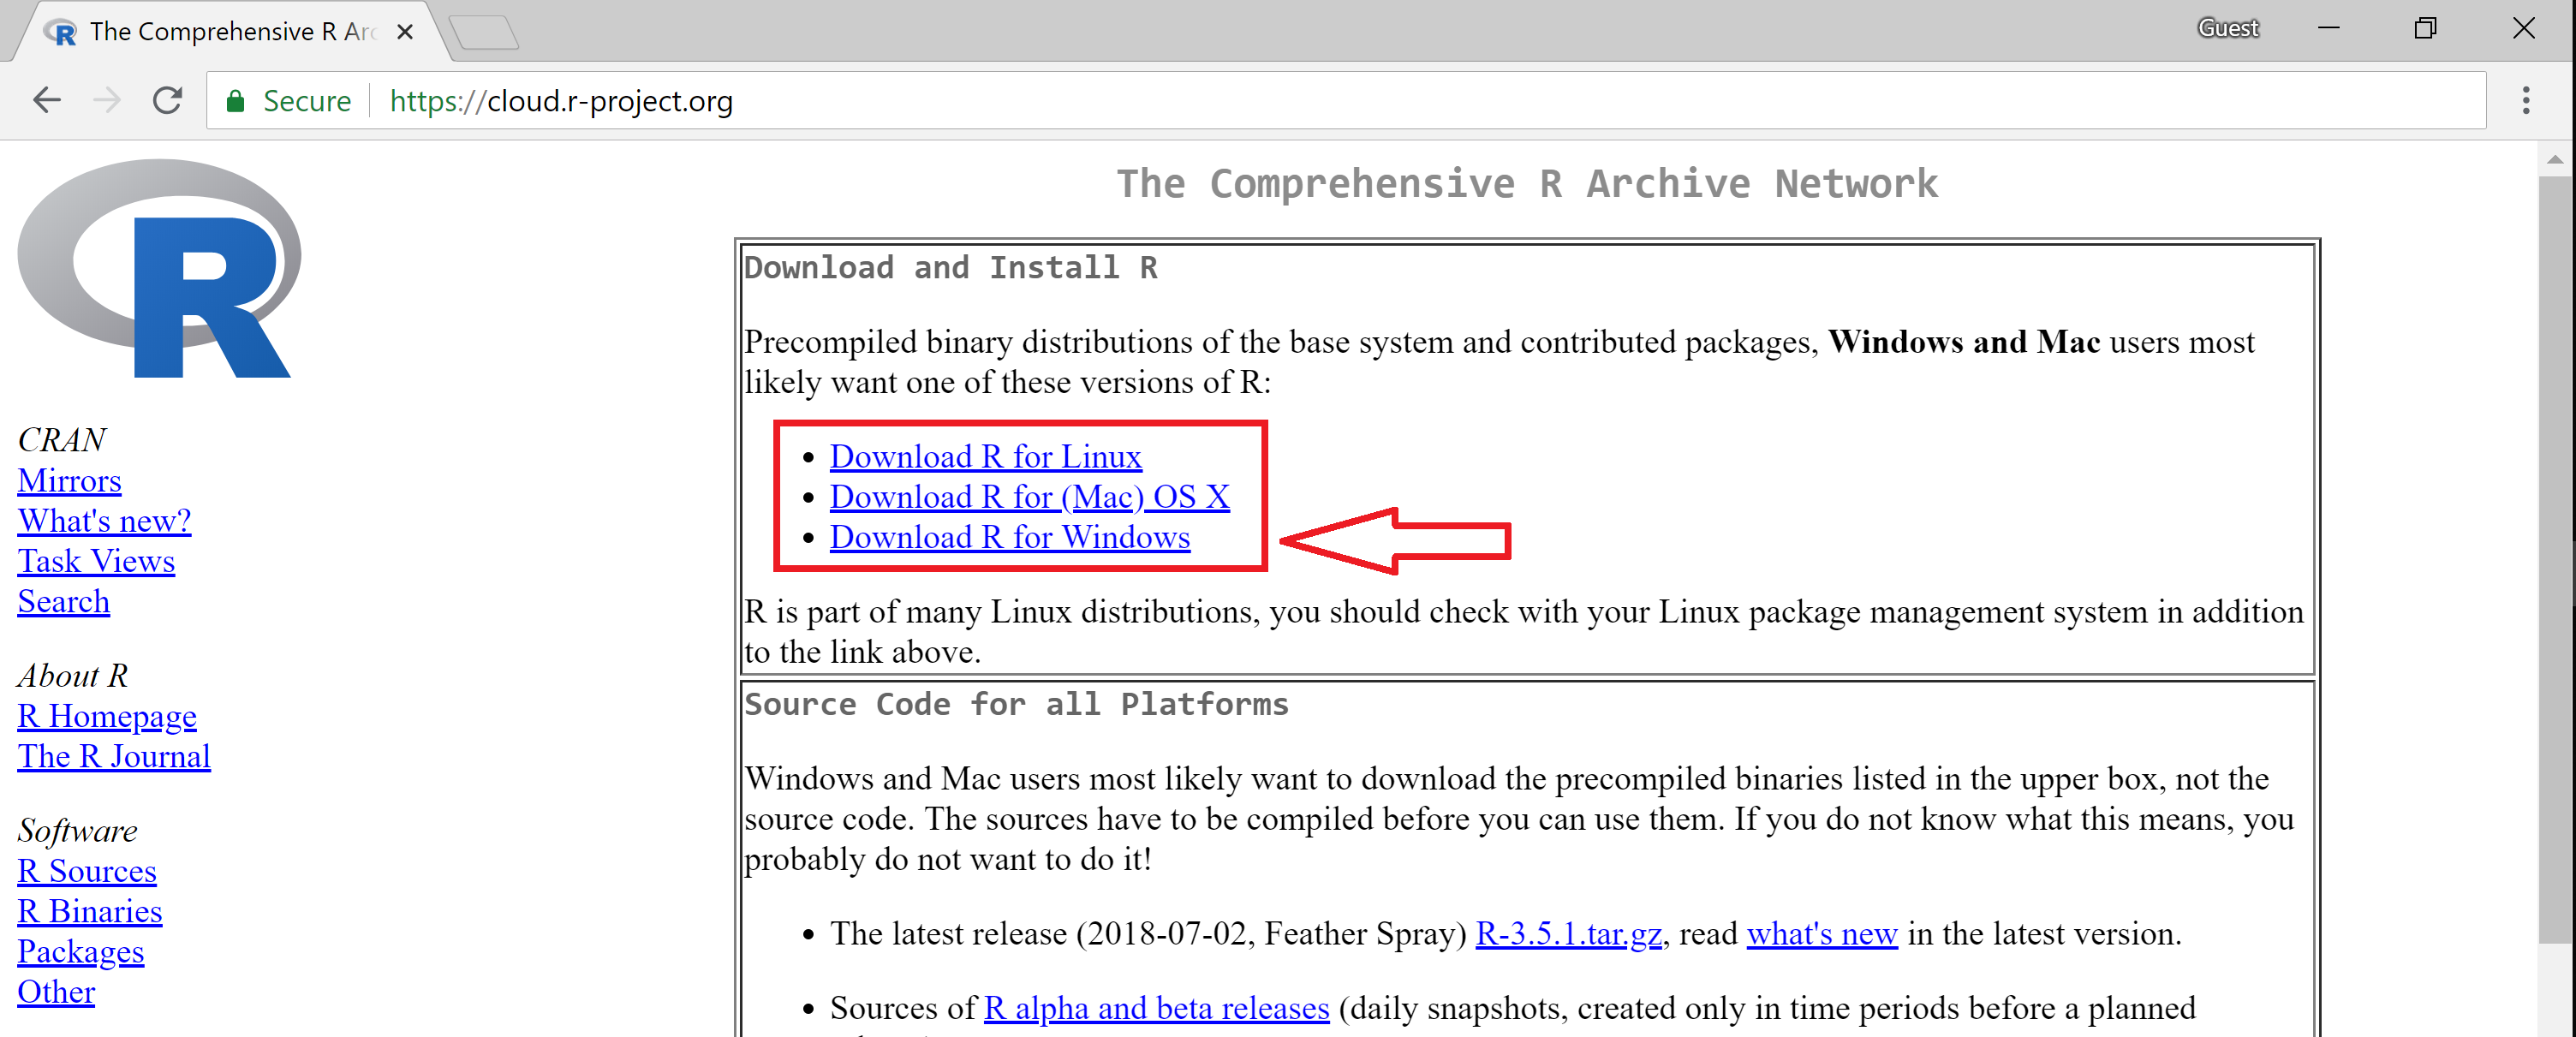
\includegraphics[width=\textwidth,height=\textheight,keepaspectratio]{./Images/image_03.png}
\end{figure}\vspace{4cm}

5) Click on the \texttt{install R for the first time}. 

\begin{figure}[!h]
 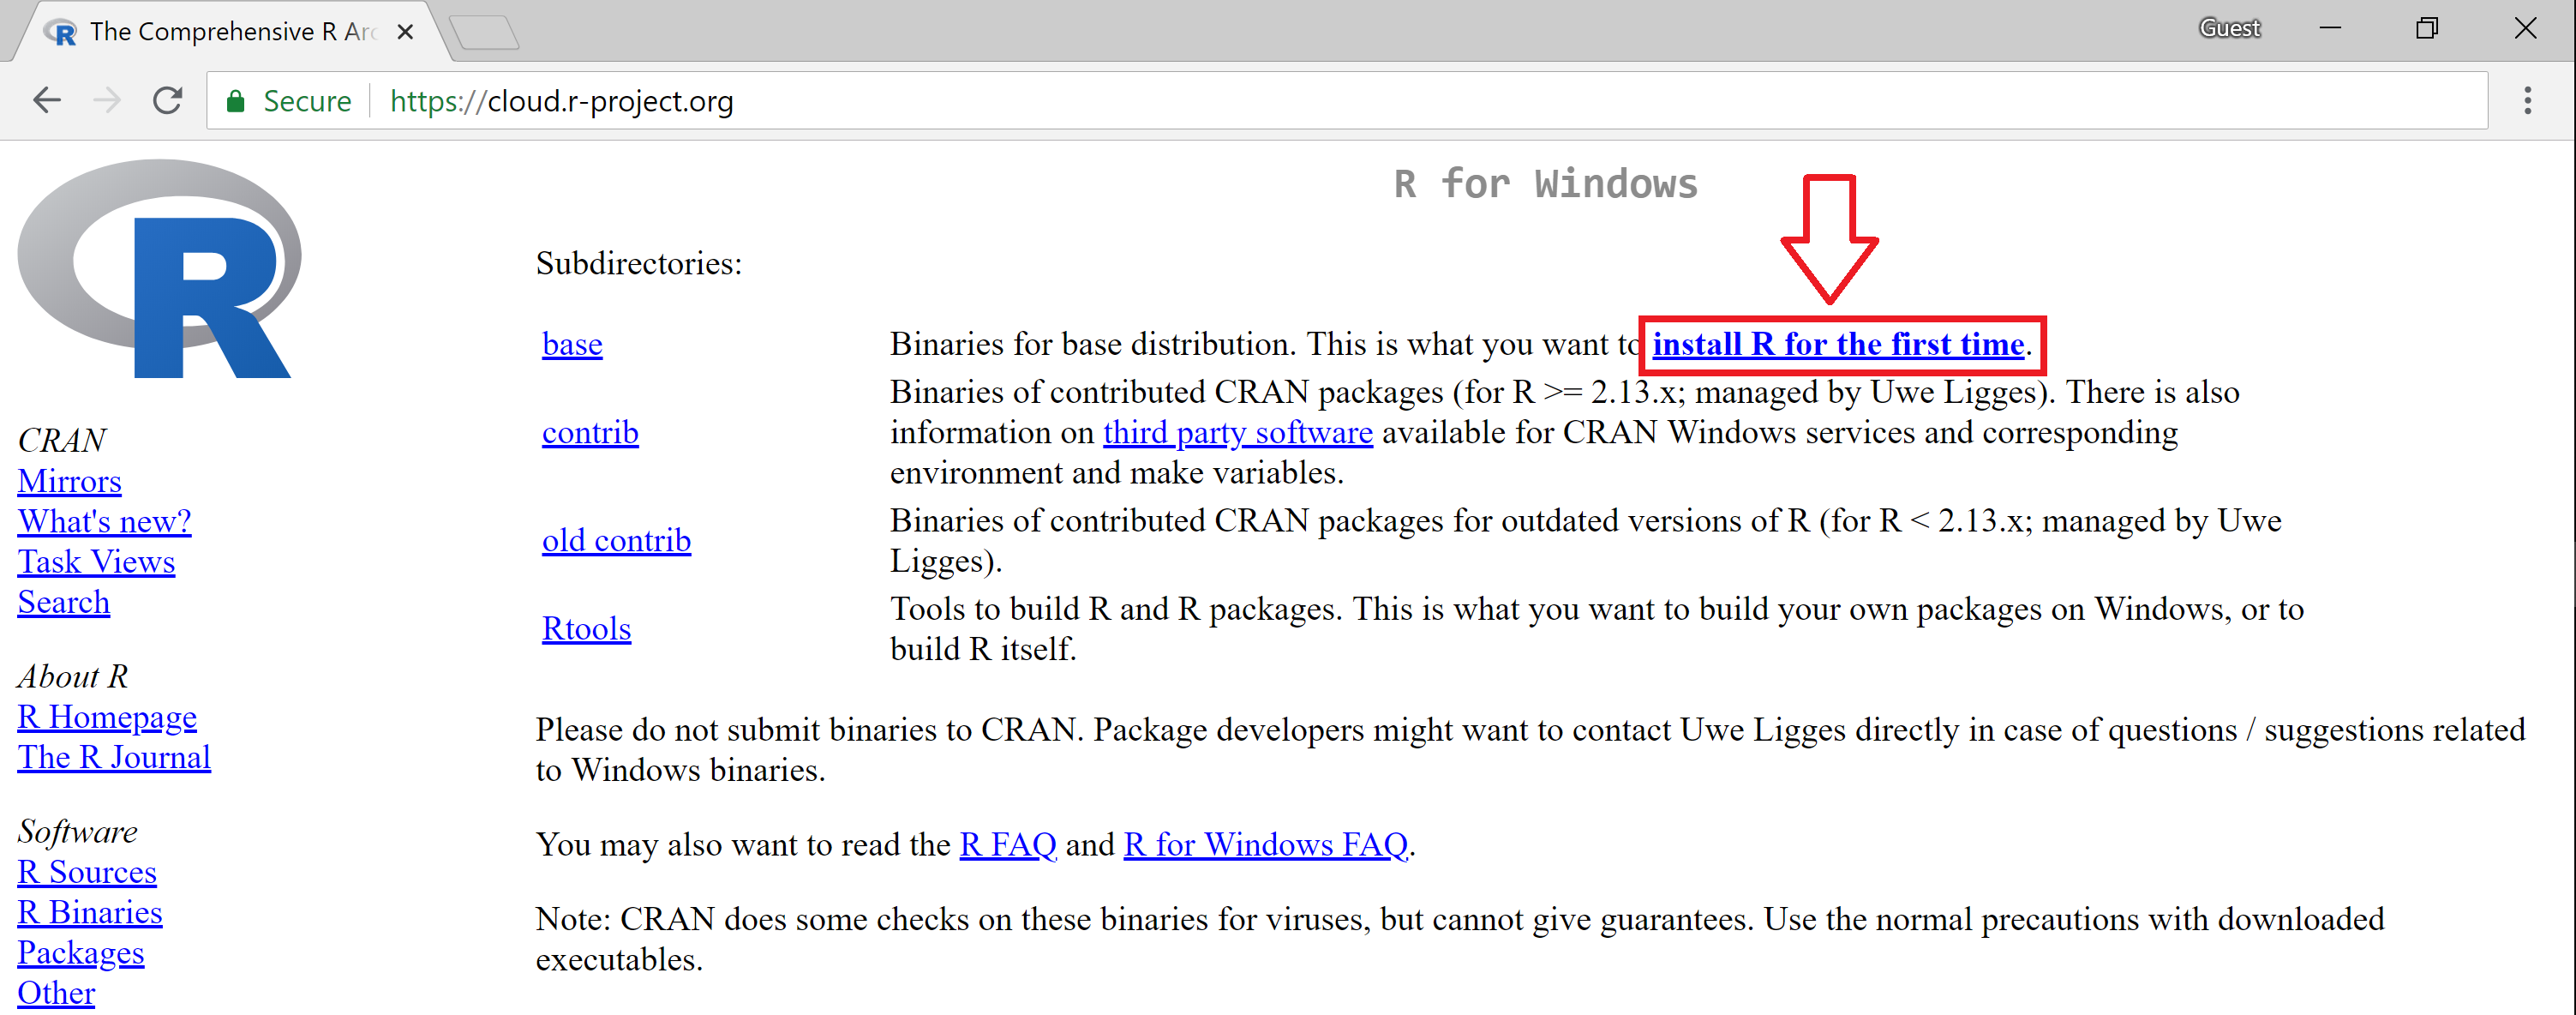
\includegraphics[width=\textwidth,height=\textheight,keepaspectratio]{./Images/image_04.png}
\end{figure}

\clearpage
6) By clicking on \texttt{Download R 3.5.1 for Windows} you initialize download.

\begin{figure}[!h]
 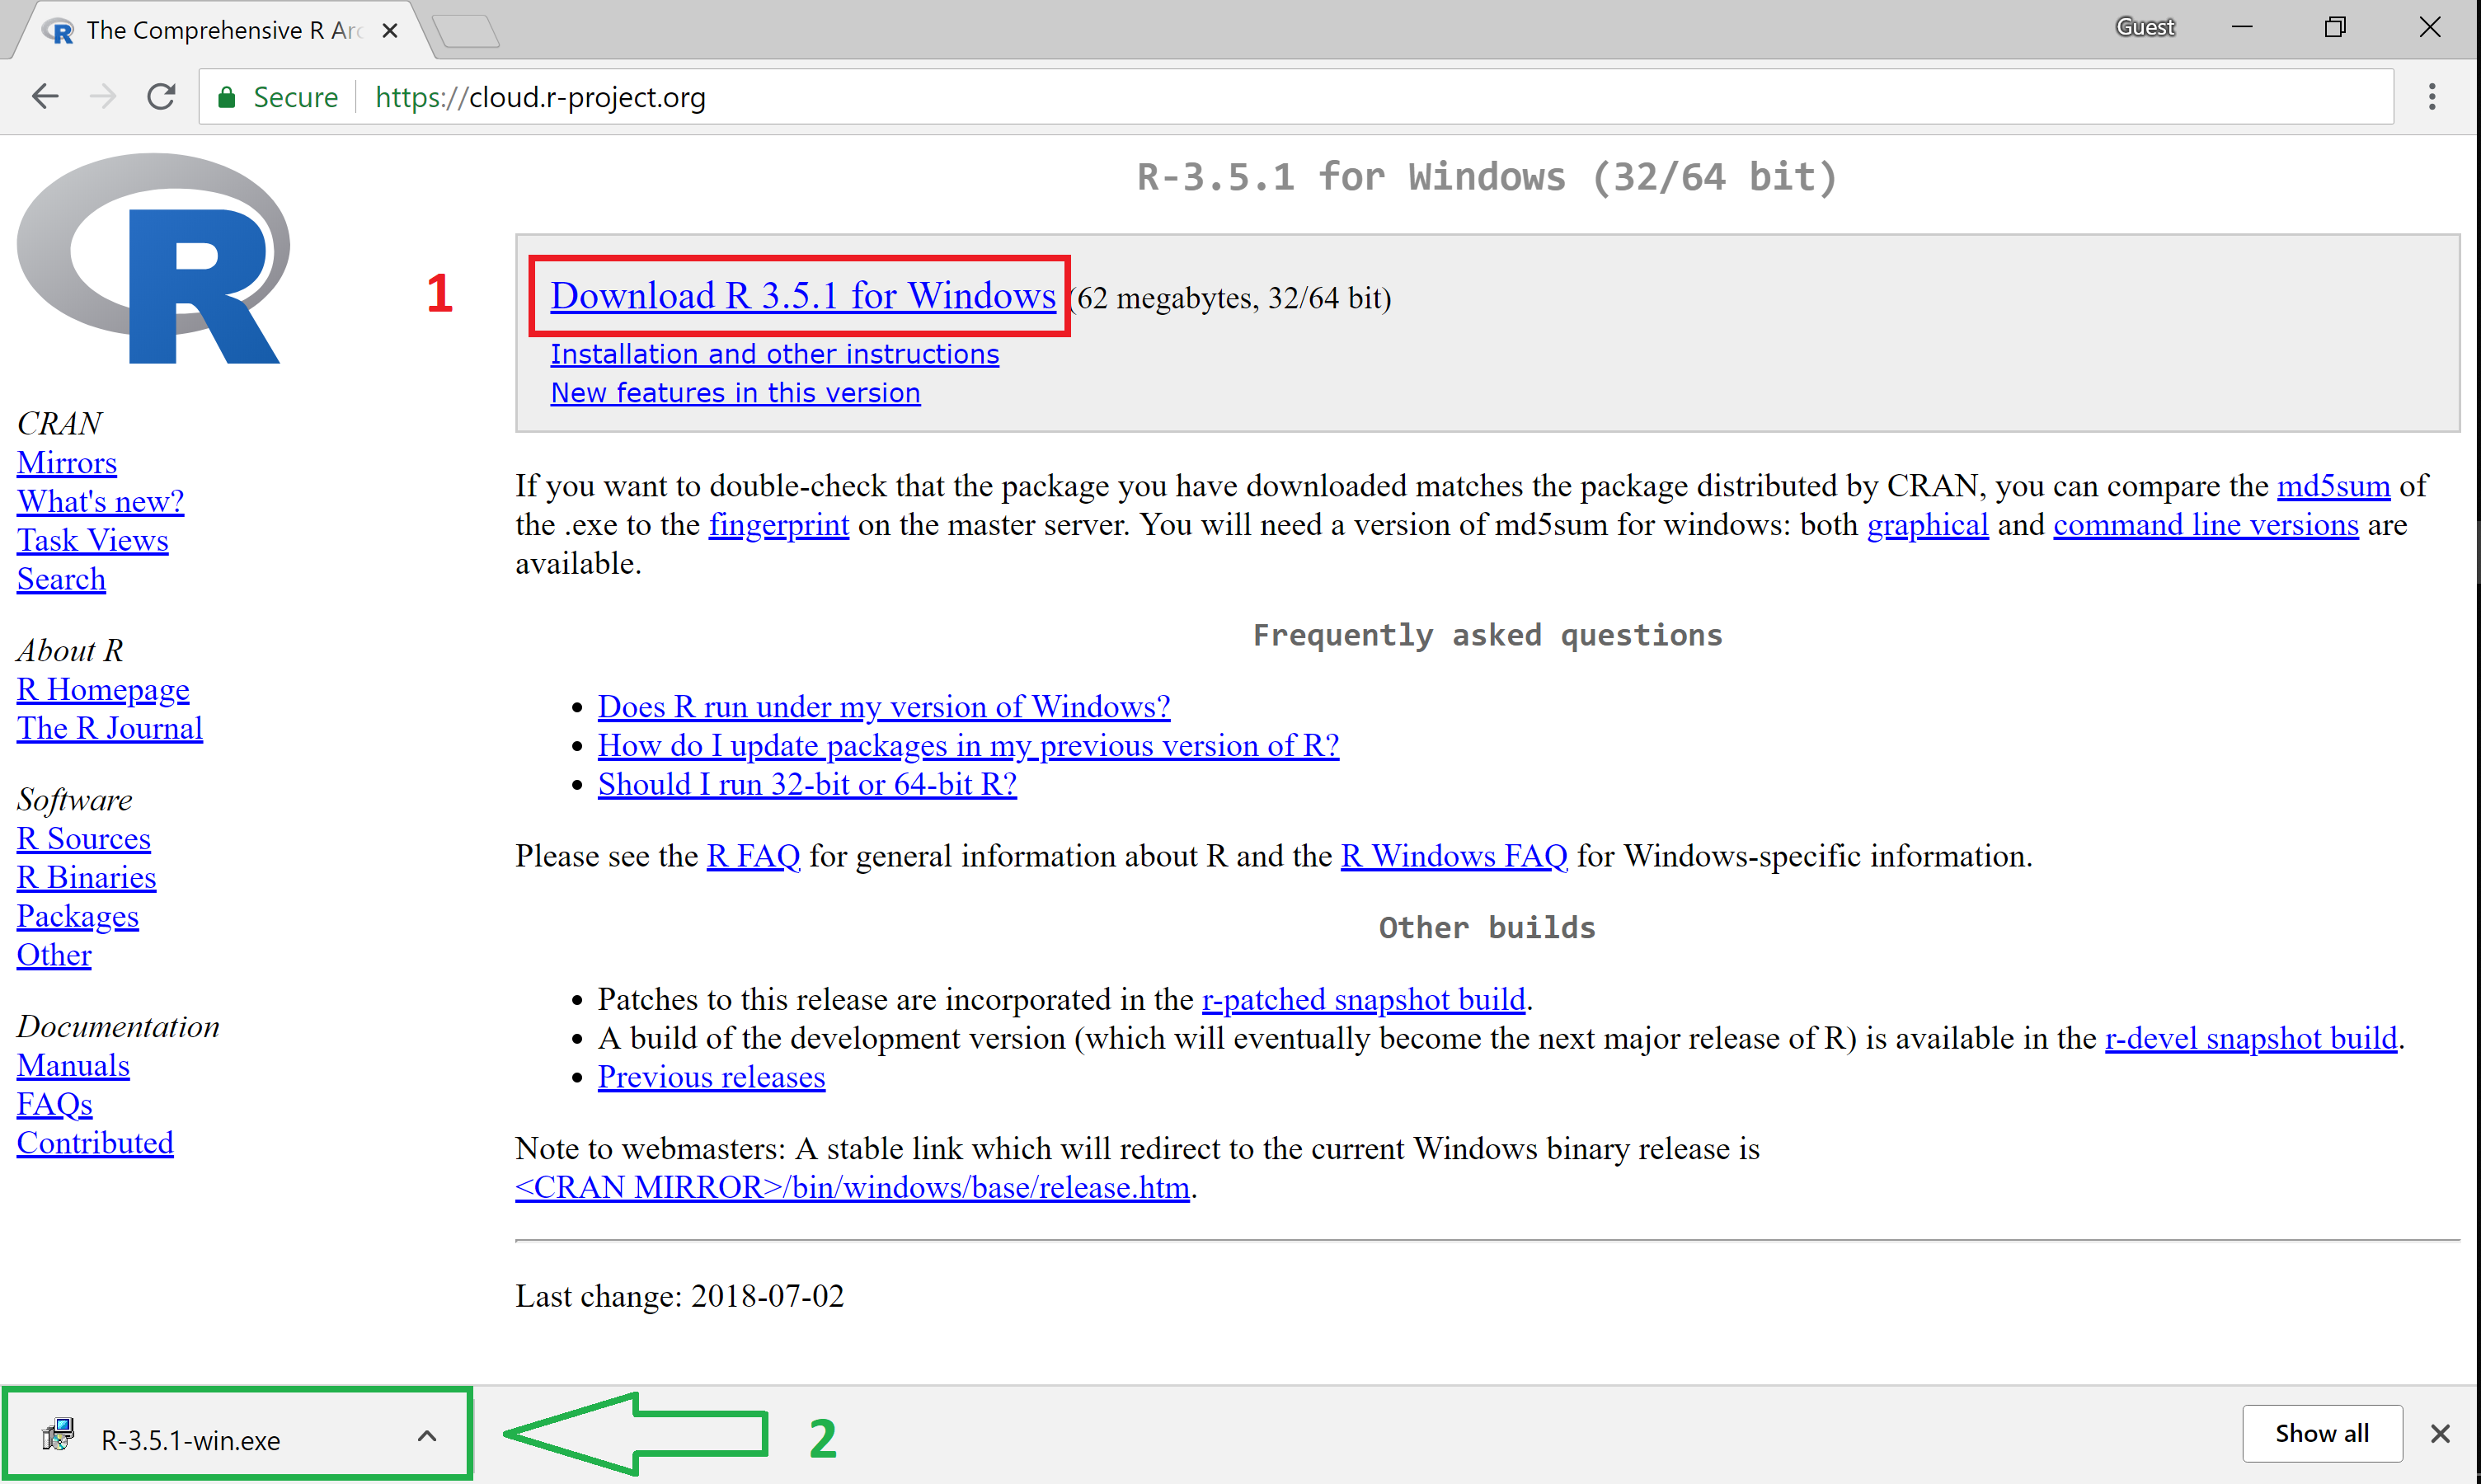
\includegraphics[width=\textwidth,height=\textheight,keepaspectratio]{./Images/image_05.png}
\end{figure}

7) Install R by running the R-3.5.1-win.exe file. Do not change anything (except of install folder, if you want to) during the installation. Just click on OK and Next.

\clearpage
\section{Configure R}
1) Locate the R icon on your desktop and run it:

\begin{figure}[!h]
 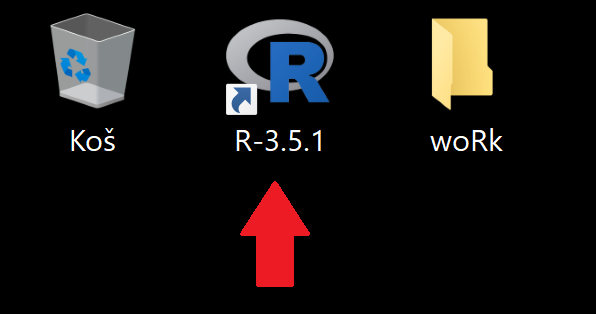
\includegraphics[scale=.5]{./Images/image_06.png}
\end{figure}

2) Copy following code:

\begin{knitrout}
\definecolor{shadecolor}{rgb}{0.969, 0.969, 0.969}\color{fgcolor}\begin{kframe}
\begin{alltt}
\hlstd{myPackages} \hlkwb{<-} \hlkwd{c}\hlstd{(}\hlstr{"tidyverse"}\hlstd{,} \hlstr{"lubridate"}\hlstd{,} \hlstr{"plotly"}\hlstd{)}
\hlkwd{install.packages}\hlstd{(myPackages)}
\end{alltt}
\end{kframe}
\end{knitrout}

and paste it into the R console:

\begin{figure}[!h]
 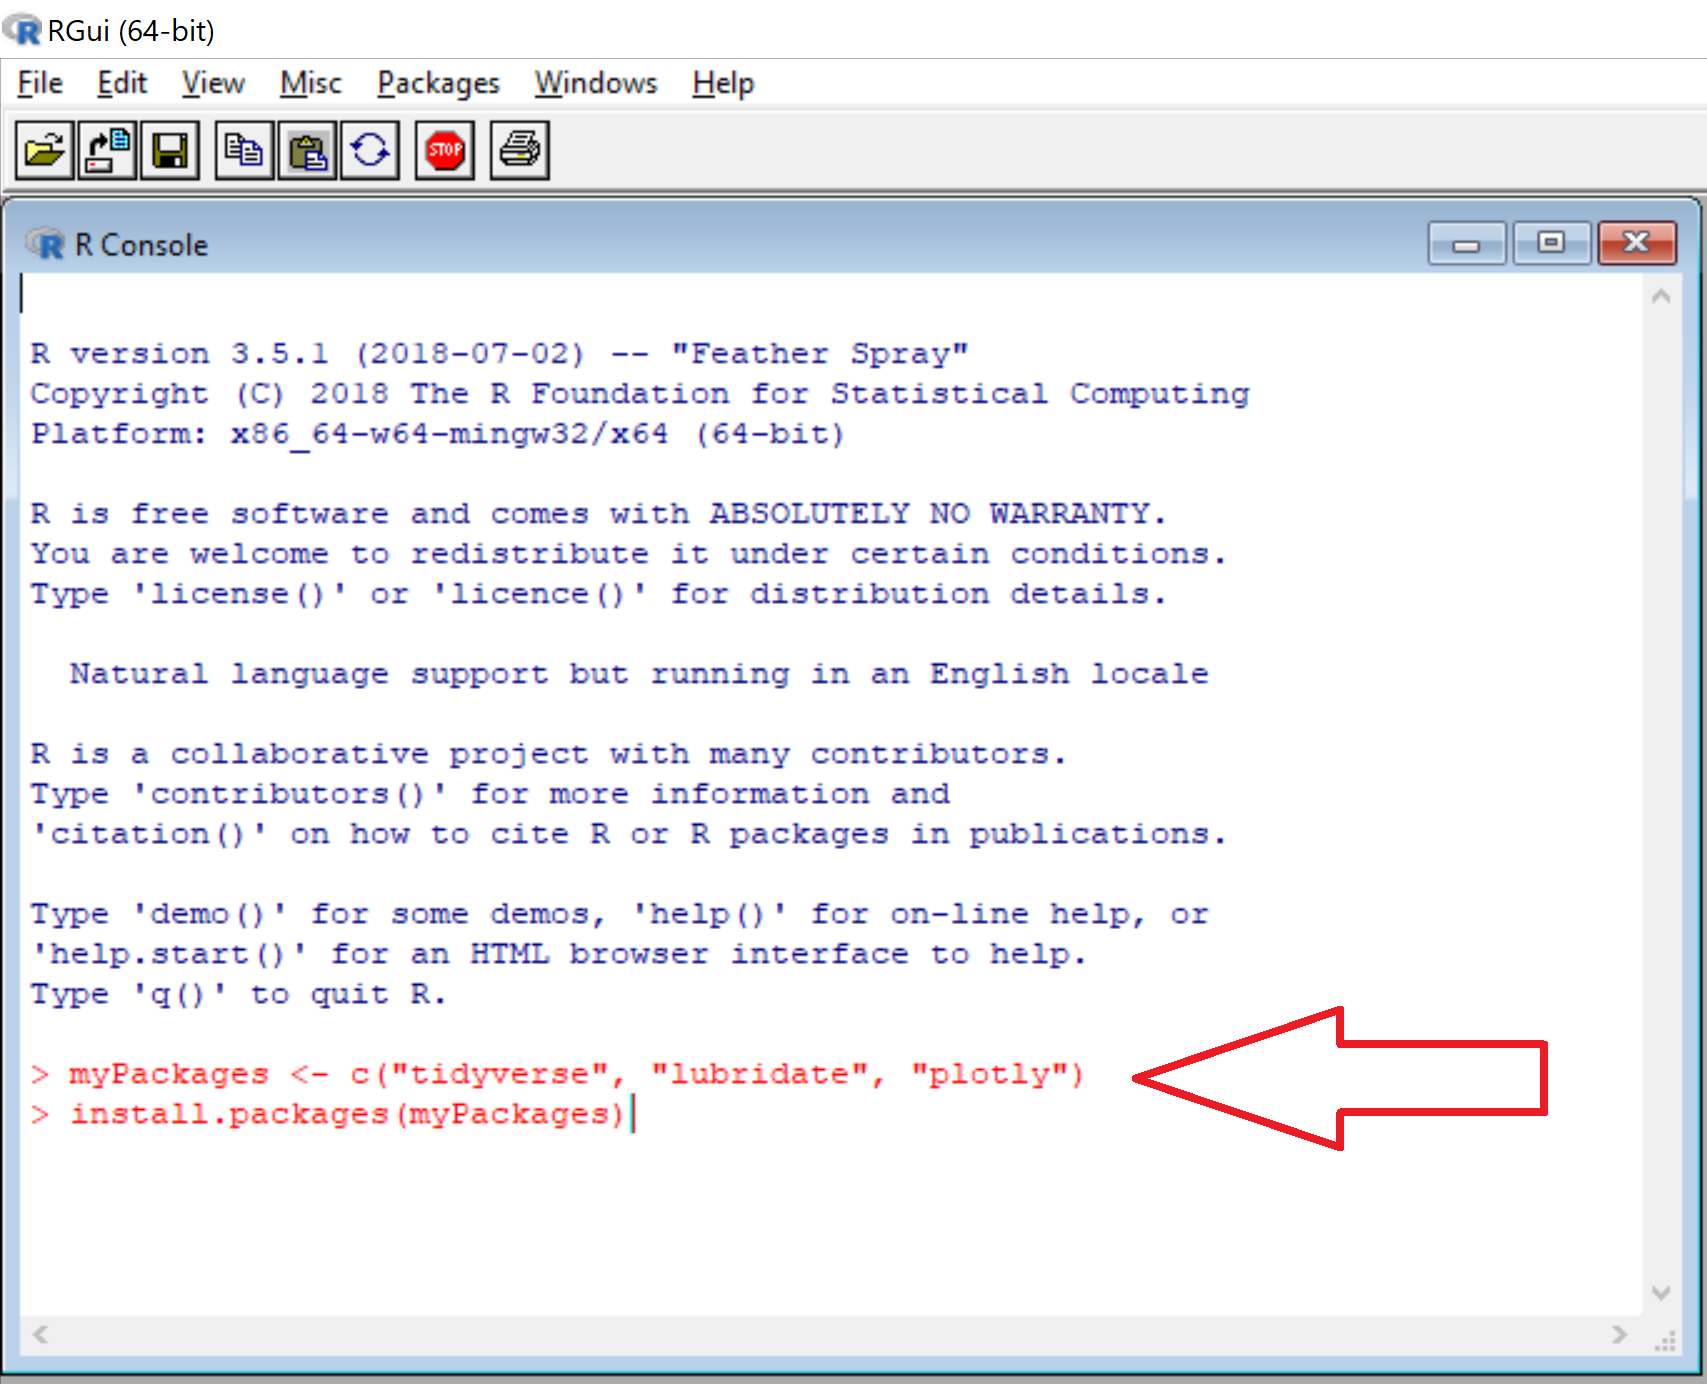
\includegraphics[width=\textwidth,height=\textheight,keepaspectratio]{./Images/image_07.png}
\end{figure}

\clearpage
3) Press Enter and select the first CRAN again. Confirm by OK.

\begin{figure}[!h]
 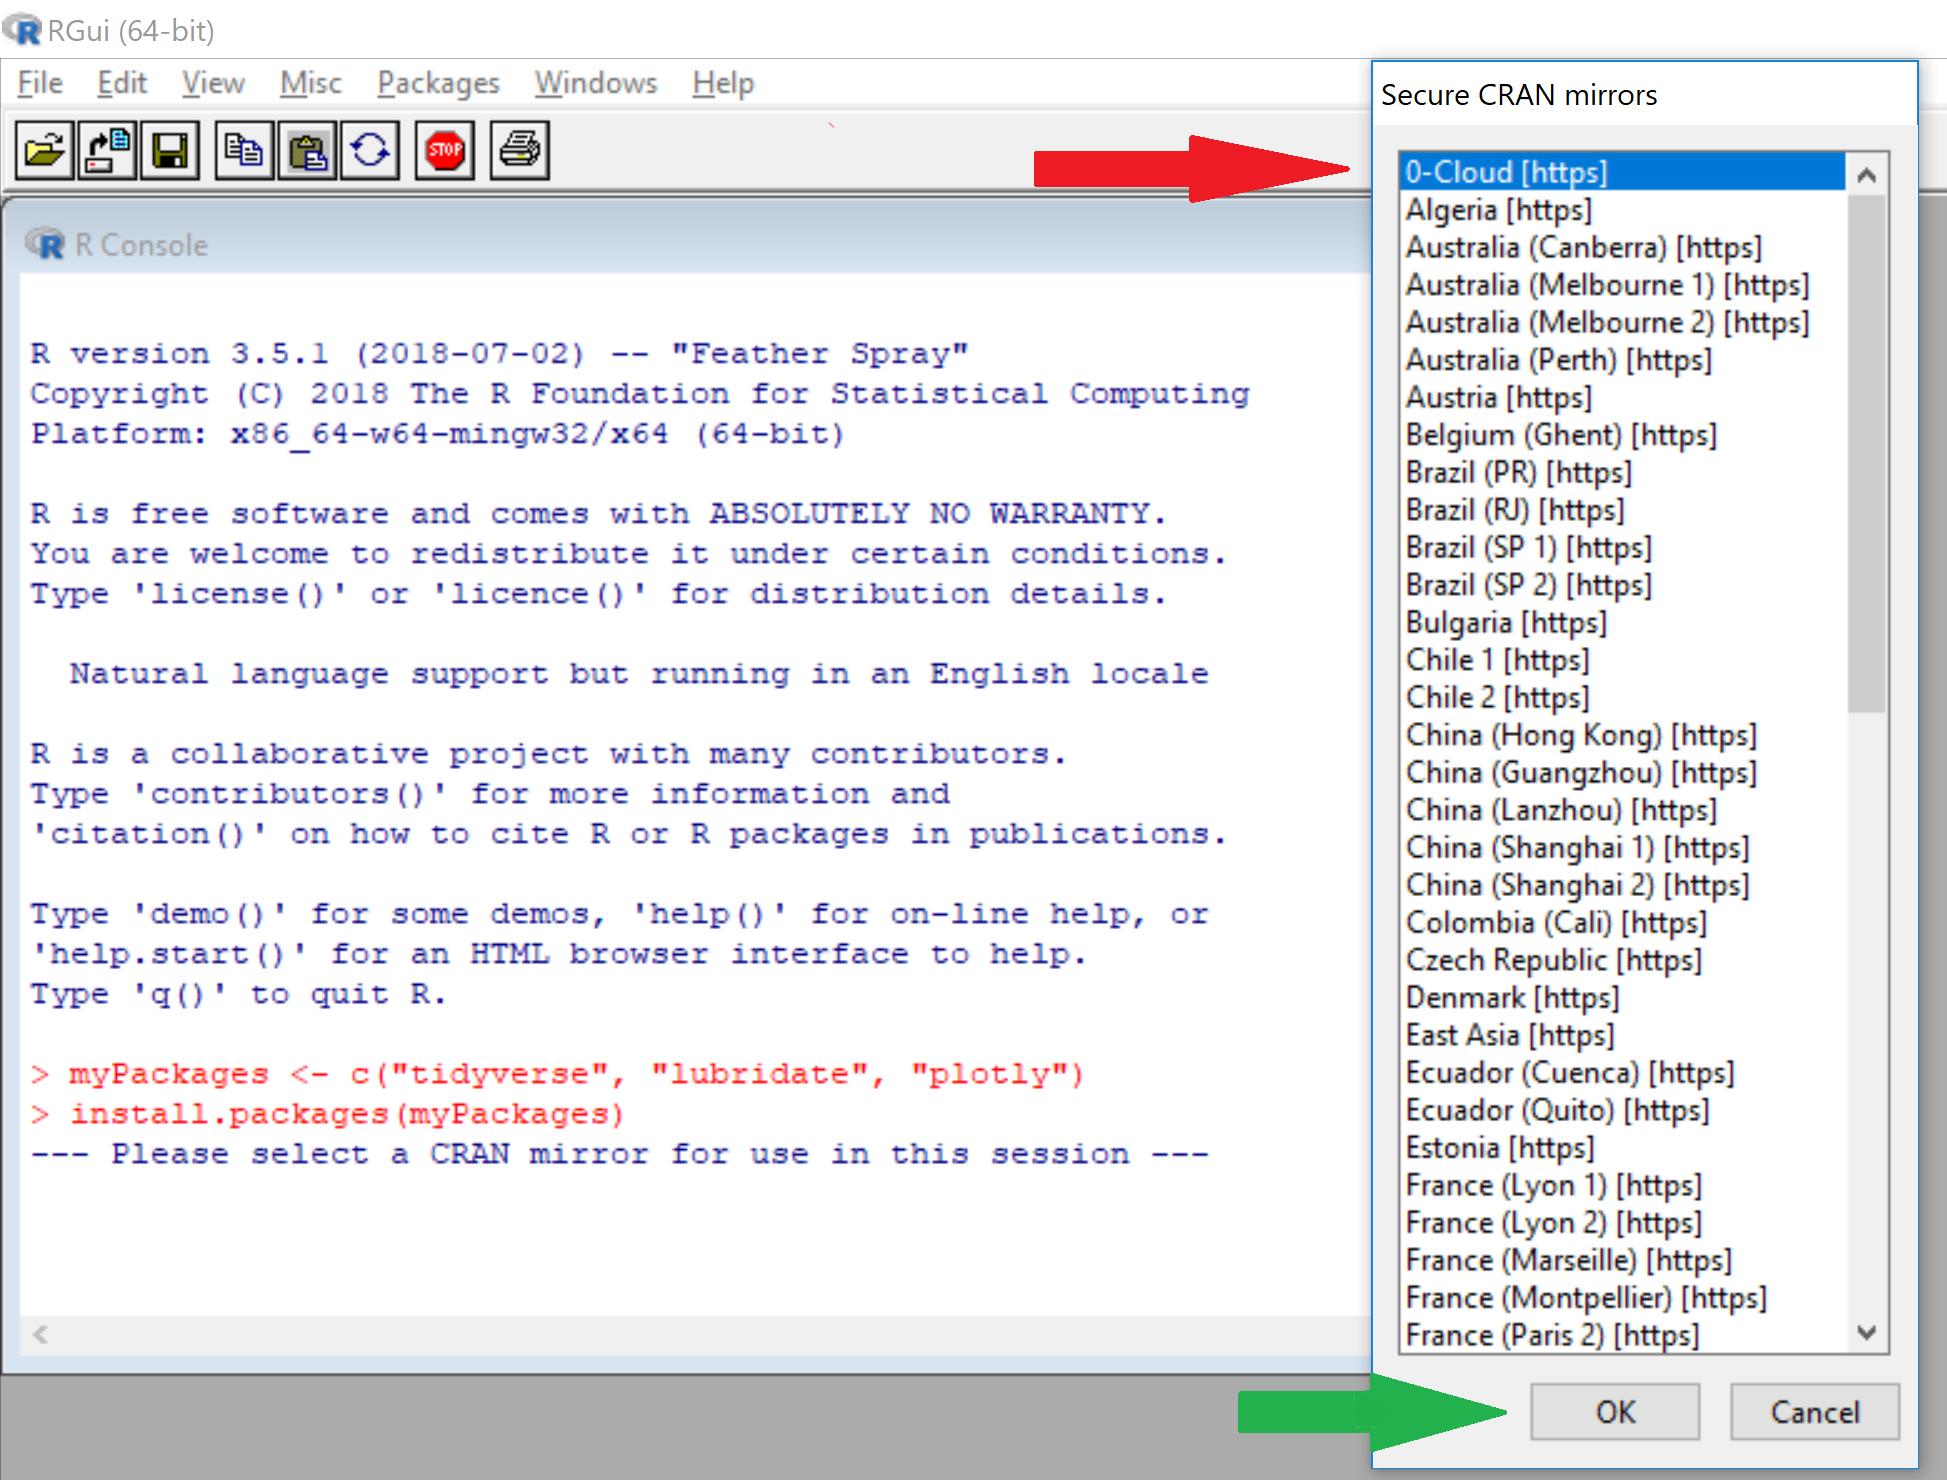
\includegraphics[width=\textwidth,height=\textheight,keepaspectratio]{./Images/image_08.png}
\end{figure} 

\clearpage
4) Run the following code (copy \& paste into the Console)
\begin{knitrout}
\definecolor{shadecolor}{rgb}{0.969, 0.969, 0.969}\color{fgcolor}\begin{kframe}
\begin{alltt}
\hlkwd{library}\hlstd{(tidyverse)}
\hlkwd{set.seed}\hlstd{(}\hlnum{123}\hlstd{)}
\hlstd{data} \hlkwb{<-} \hlkwd{data.frame}\hlstd{(}\hlkwc{x}\hlstd{=}\hlkwd{rnorm}\hlstd{(}\hlnum{100}\hlstd{),} \hlkwc{y}\hlstd{=}\hlkwd{rnorm}\hlstd{(}\hlnum{100}\hlstd{))}
\hlkwd{ggplot}\hlstd{(data,} \hlkwd{aes}\hlstd{(x,y) )} \hlopt{+}
 \hlkwd{geom_point}\hlstd{(}\hlkwc{alpha}\hlstd{=}\hlnum{0.8}\hlstd{)}
\end{alltt}
\end{kframe}
\includegraphics[width=\maxwidth]{figure/unnamed-chunk-2-1} 

\end{knitrout}

Do you see the figure above? Great, you are ready to attend the workshop! If you have encountered any trouble during this guide, please contact me at {\color{blue} homolka@utb.cz}. \bigskip

5) Close R. Don't save your workspace.

\begin{figure}[!h]
 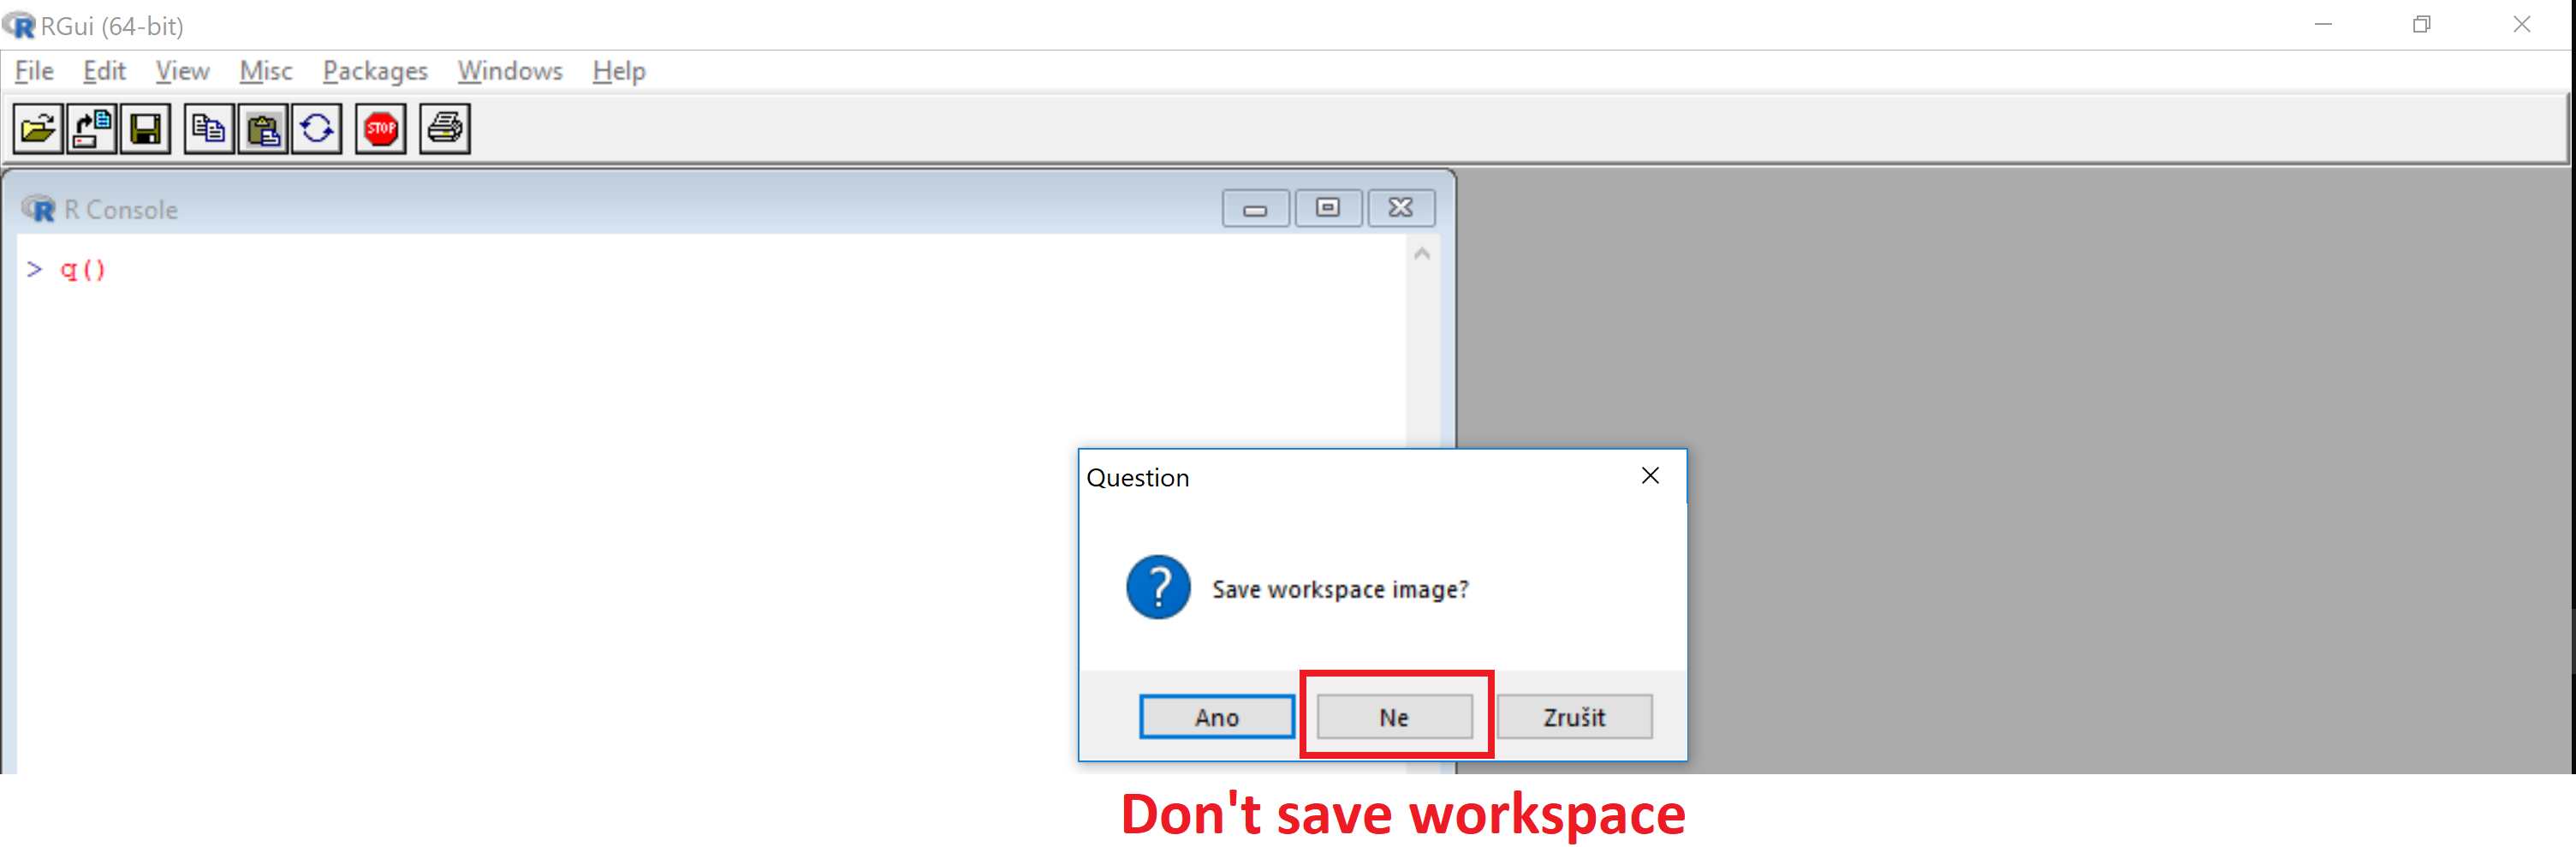
\includegraphics[width=\textwidth,height=\textheight,keepaspectratio]{./Images/image_09.png}
\end{figure}

\end{document}
